\documentclass[11pt,a4paper]{article}
\usepackage[style=apa,autocite=inline]{biblatex}
\addbibresource{ref.bib}
\usepackage[margin=3.5cm]{geometry}
\usepackage[utf8]{inputenc}
\usepackage[parfill]{parskip}
\usepackage{graphicx}
\usepackage{float}
\usepackage[width=0.8\textwidth]{caption}
\usepackage{csquotes}
\usepackage{amsmath}
\usepackage{amssymb}
\usepackage{amsthm}
\usepackage{verbatim}
\providecommand{\keywords}[1]{\textbf{\textit{Keywords:}} #1}
\usepackage{pgfplots}
\pgfplotsset{compat=1.16}
\usepgfplotslibrary{fillbetween}
\usepackage[hypertexnames=false]{hyperref}
\usepackage{subcaption}
\usepackage[normalem]{ulem}
\usepackage{texshade}
\usepackage{multirow}
\usepackage[affil-it]{authblk}
\usepackage[bottom]{footmisc}
\def\@fnsymbol#1{\ensuremath{\ifcase#1\or \dagger\or \ddagger\or
   \mathsection\or \mathparagraph\or \|\or **\or \dagger\dagger
   \or \ddagger\ddagger \else\@ctrerr\fi}}

\newcommand\blfootnote[1]{%
  \begingroup
  \renewcommand\thefootnote{}\footnote{#1}%
  \addtocounter{footnote}{-1}%
  \endgroup
}

\title{\textit{In vitro} mutagenesis of pHis$_6$-Z-(stop)-mCherry plasmid in \textit{E. coli}}
\author{Hans Jiang\thanks{001006-0077, hansji@kth.se} $\: \:$Elin Lenart\thanks{990628-1945, elenart@kth.se}$\: \:$}
\date{April 2020}


\begin{document}
\maketitle
\pagenumbering{gobble}

\begin{abstract}
Site-directed mutagenesis is a mutation introduced to the genetic material in an organism. It is a standard technique in the field of biotechonology. In this lab the His$_6$-Z-(stop)mCherry resistance plasmid in \textit{E. coli} was mutated by removing the stop codon: TAA $\rightarrow$ CAA, thence enabling translation of the mCherry fluorecent domain. This was done in multiple steps, including analyses to along the process: extraction and purification of the plasmid, mutagenesis by PCR, heat shock mediated transformation and finally incubation in selective ampicillin media. Plasmid concentration was measured after extraction. PCR and gel electrophoresis, sanger sequencing and protein analysis with SDS-PAGE after incubation. Incubation showed a result of 11 \% mutation frequency. Results of the analytical steps were mostly expected. \blfootnote{Group number: 24} \blfootnote{Peer-review by: Daniel Ullman, Simona Pettersson} \\

%Detta är 195 ord: Lorem ipsum dolor sit amet, consectetur adipisicing elit, sed do eiusmod tempor incididunt ut labore et dolore magna aliqua. Ut enim ad minim veniam, quis nostrud exercitation ullamco laboris nisi ut aliquip ex ea commodo consequat. Duis aute irure dolor in reprehenderit in voluptate velit esse cillum dolore eu fugiat nulla pariatur. Excepteur sint occaecat cupidatat non proident, sunt in culpa qui officia deserunt mollit anim id est laborum. Lorem ipsum dolor sit amet, consectetur adipisicing elit, sed do eiusmod tempor incididunt ut labore et dolore magna aliqua. Ut enim ad minim veniam, quis nostrud exercitation ullamco laboris nisi ut aliquip ex ea commodo consequat. Duis aute irure dolor in reprehenderit in voluptate velit esse cillum dolore eu fugiat nulla pariatur. Excepteur sint occaecat cupidatat non proident, sunt in culpa qui officia deserunt mollit anim id est laborum. Lorem ipsum dolor sit amet, consectetur adipisicing elit, sed do eiusmod tempor incididunt ut labore et dolore magna aliqua. Ut enim ad minim veniam, quis nostrud exercitation ullamco laboris nisi ut aliquip ex ea commodo consequat. Duis aute irure dolor in reprehenderit in voluptate velit esse cillum dolore eu fugiat nulla pariatur. Lorem ipsum, dolor sit amet, cons.
\end{abstract}
\keywords{pHis$_6$-Z-(stop)-mCherry, \textit{in vitro} mutagenesis, \textit{E. coli}}
\pagebreak
\tableofcontents \pagebreak

\pagenumbering{arabic}
\setcounter{page}{1}

\section{Introduction}
Genes are what govern a cells’ behaviour by controlling what proteins and in what amount they are produced  in response to internal signals or external stimuli. Site directed mutagenesis means to make a change in a gene of a cell at a specific site. Site specificity is very important as "mutagenesis" simply means a change to the genome, whether intentional or non-intentional, useful or harmful. An example would be cancer which is both a non-intentional and harmful instance(s) of mutagenesis. Site-specifically introduced mutation is a very important technique in biotechnology to study the role of a gene or to change a property thereof to our use. The former can be done by introducing a nonsense mutation (or cut out entirely) to see how the organism responds, this is called a "knock-out". The latter is used in a myriad of different settings; for example in industrial and medical applications by altering the expression rate or the property of the relevant protein. In bacteria, this is done quite easily on a plasmid by first extracting it, introducing the mutation \textit{in vitro} and transforming them back into the bacteria. A popular method of doing said point mutation is the QuickChange procedure, where a mutation is introduced through a nucleic acid with a mismatched primer. In this lab, mutagenesis was done in \textit{E. coli} in the resistance plasmid pHis$_6$-Z-stop-mCherry by removing the stop codon, thereby enabling transcription and translation of the fluorecent mCherry protein domain. To check success of mutagenesis and transformation, targeted PCR and sequencing and protein analysis by SDS-PAGE was done. 
%----------------------------------------------------------------------------------------
\section{Methodology}
%lägger till subsections men jag tror inte de vill ha det. Vi tar bort det senare, jag kan inte se annars
\subsection{Plasmid extraction and purification}
The His$_6$-Z-(stop)-mCherry plasmid was extracted and purified from a pellet of \textit{E. coli} cells. First, the pellet was suspended in 250 $\mu$L P1 buffer. P2 buffer (250 $\mu$L) following N3 buffer (350 $\mu$L) was added and inverted after each addition. This solution was centrifuged for 10 min at 13000 rpm. 750 $\mu$L of the supernatant from the tube was transferred to a QIAquick spin column, which was centrifuged at 13000 rpm for 1 min. The supernatant was discarded and 750 $\mu$L of PE buffer was added. The sample was centrifuged for 1 min 13000 rpm, and the flow through was discarded. The sample was centrifuged for 1 min at same, and eventual flow through of remaining PE buffer was discarded. The column was transferred to a 1.5 mL Eppendorf tube, filled with 50 $\mu$L EB-buffer and incubated at room temperature for 1 min before being centrifuged for 1 min at 13000 rpm. The flow through was saved for later use.

\subsection{Gel electrophoresis of purified plasmid DNA}

The concentration and purity of the plasmid were determined via gel electrophoresis. Two samples were made: A and B. To both, MilliQ (4 $\mu$L) and 6x concentrated loading dye (1 $\mu$L) were added. Undiluted plasmid mixture was added to A and 1:10 diluted plasmid mixture was added to B. 5 $\mu$L of samples A and B were loaded in an electrophoresis setup in 1\% agarose gel containing GelRed. The electrophoresis ran at 150 V for 40 min. The gel slab was put under UV light to illuminate the DNA. The DNA concentration was measured with a NanoDrop spectrometer by the lab assistants.

\subsection{Mutagenesis}
The plasmid was mutated \textit{in vitro}. The following parts of PCR solution were added to an Eppendorf tube, with the DNApol last: plasmid DNA (4.1 $\mu$L giving 700 ng), dNTPs (2mM of each dNTP)(5 $\mu$L), forward primer solution (5 pmol/$\mu$L)(2.6 $\mu$L), reverse primer solution (5 pmol/$\mu$L) (2.6 $\mu$L), 5x HF buffer (10 $\mu$L), MilliQ (24.7 $\mu$L), Phusion DNApol (2 U/$\mu$L) (1 $\mu$L). The total volume was 50 $\mu$L. The sample was run in PCR according to this profile: $$1*[98 \: ^{\circ}C \: 30 \: \textrm{s}], \: 12*[98 \: ^{\circ}C \: 30 \: \textrm{s}, \: 55 \: ^{\circ}C \: 1 \: \textrm{min}, 72 \: ^{\circ}C \: 3.5 \: \textrm{min}], 1*[4 \: ^{\circ}C]$$
Next, the following were added to an Eppendorf tube: mutagenesis mixture (40 $\mu$L), 10x CutSmart buffer (5 $\mu$L), MilliQ (4.5 $\mu$L), \textit{Dpn}I enzyme (2 U/$\mu$L) (0.5 $\mu$L). This digestion mixture was incubated at 37 $^\circ C$ for 20 min. 

\subsection{Transformation}
The \textit{E. coli} cells were transformed by heat shock. 50 $\mu$L of competent cells were mixed with 40 $\mu$L of the previously prepared plasmid solution. It was mixed and kept on ice for 20 minutes. Next, the sample was incubated at 42 $^\circ C$ for 50 s (heat shock), then put on ice for 3 min. 200$\mu$L of LB liquid media was added and incubated while shaken at 37 $^\circ C$ for 45 min. 200$\mu$L of this solution was added to (racklad) an agar plate with ampicillin (100 $\mu$g/mL) and incubated at 37 $^\circ C$ overnight. The plate was examined.

\subsection{PCR of colonies}
4.8 $\mu$L PCR-buffer, 4.8 $\mu$L dNTP-mix (2 mM), 4.8 $\mu$L "F\_PCR" forward primer (5 $\mu$M), 4.8 $\mu$L "R\_PCR" reverse primer (5 $\mu$M), 0.48 $\mu$L \textit{Taq} DNA-polymerase (5 U/$\mu$L), 28.32 $\mu$L MilliQ in two marked 1.5 mL Eppendorf tubes. One purple and white colony was individually suspended in 20 $\mu$L of MilliQ. 2 $\mu$L of respective suspension was transferred to separate marked tubes containing the prepared PCR solution.  Each mixture was run in PCR according to following profile: $$1*[94 \: ^{\circ}C \: 5 \: \textrm{min}], \: 25*[94 \: ^{\circ}C \: 20 \: \textrm{s}, \: 65 \: ^{\circ}C \: 30 \: \textrm{s}, 72 \: ^{\circ}C \: 1 \: \textrm{min}], 1*[72 \: ^{\circ}C\: 5 \: \textrm{min}]$$

\subsection{Gel electrophoresis on PCR product}
The length of the plasmid was determined with gel electrophoresis. The samples were prepared: PCR product (from white and red colonies) (3 $\mu$L), loading dye (1 $\mu$L) and MilliQ (2 $\mu$L) ($\sum$ 6 $\mu$L). 5 $\mu$L of prepared mixtures along with pre-prepared molecular markers were added to each well. Electrophoresis was run in 150 V for \linebreak 40 min and visualized with UV light.

\subsection{Sanger sequencing}
The sequence was sent to be sequenced externally.

\subsection{Protein production}
The white and red cultures were inoculated in separate 10 mL liquid LB media containing 0.101 mL ampicillin (100 $\mu$g/mL)(Appendix E) overnight at 37 $^\circ C$ while shaking \linebreak(150 rpm). 

\subsection{Analysis of protein by SDS-PAGE}
25 $\mu$L of purple and white colony suspension were added to 125 $\mu$L reducing buffer added in two separate tubes. These were boiled for 5 minutes at 95 $^\circ C$. 20 $\mu$L of each sample and 5 $\mu$L of LMW ladder were loaded in an agar gel slab and electrophoresis was run for 60 min at 200 V. Resulting gel was stained and scanned.

%-------------------------------------------------------------------------------------------
\section{Results and conclusions}
 \subsection{Plasmid purification}
Three bands are very apparent on the lanes for both sample A and B. At the upper half of lane A, there are a multiple of other faint bands showing. The three strongly lit bands result from the three main structural forms that the His$_6$-Z-(stop)mCherry can have, being circular, super-coiled and linear. The three forms interact with the gel differently and therefore run at different speed. The size of the pHis$_6$-Z-(stop)-mCherry plasmid is approximately 3500 bp, so the band between the third and fourth band on the “High DNA mass ladder” (counted from the top) is likely to be the linear version of the plasmid. 

The lowest band in the DNA mass ladder represents a concentration of 10 ng/$\mu$L, and the upmost band a concentraiton of 100 ng/$\mu$L. When compared to the DNA mass ladder, the band of interest from sample B is estimated to be less than 10 ng/$\mu$L. Similarly, the band from sample A is indicating a concentration at around 100 ng/$\mu$L. The concentration of DNA in sample A of the relevant plasmid is 170 ng/$\mu$l according to absorbance test with NanoDrop. 

\begin{figure}[H]
    \centering
    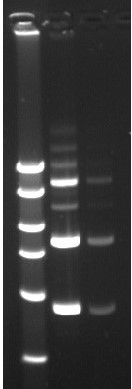
\includegraphics[scale=0.45]{Plasmid_Gel_Zoom_GeDoc 2020-03-31_13h00m41s.jpg}
    \caption{UV analysis of the gel electrophoresis with samples (from the left): DNA ladder, sample “A”, sample “B”}
    \label{fig1}
\end{figure}

 \subsection{Transformation}
The colonies in Fig. 2 were counted, see calculation in Appendix B. The transformed colonies are indicated by their pink color which comes from the mCherry protein domain. 11 \% is a low transformation frequency. It is unclear why the right side of the agar plate has visibly less colonies; the cell suspension was streaked evenly and the agar was homogeneous.

\begin{figure}[H]
    \centering
    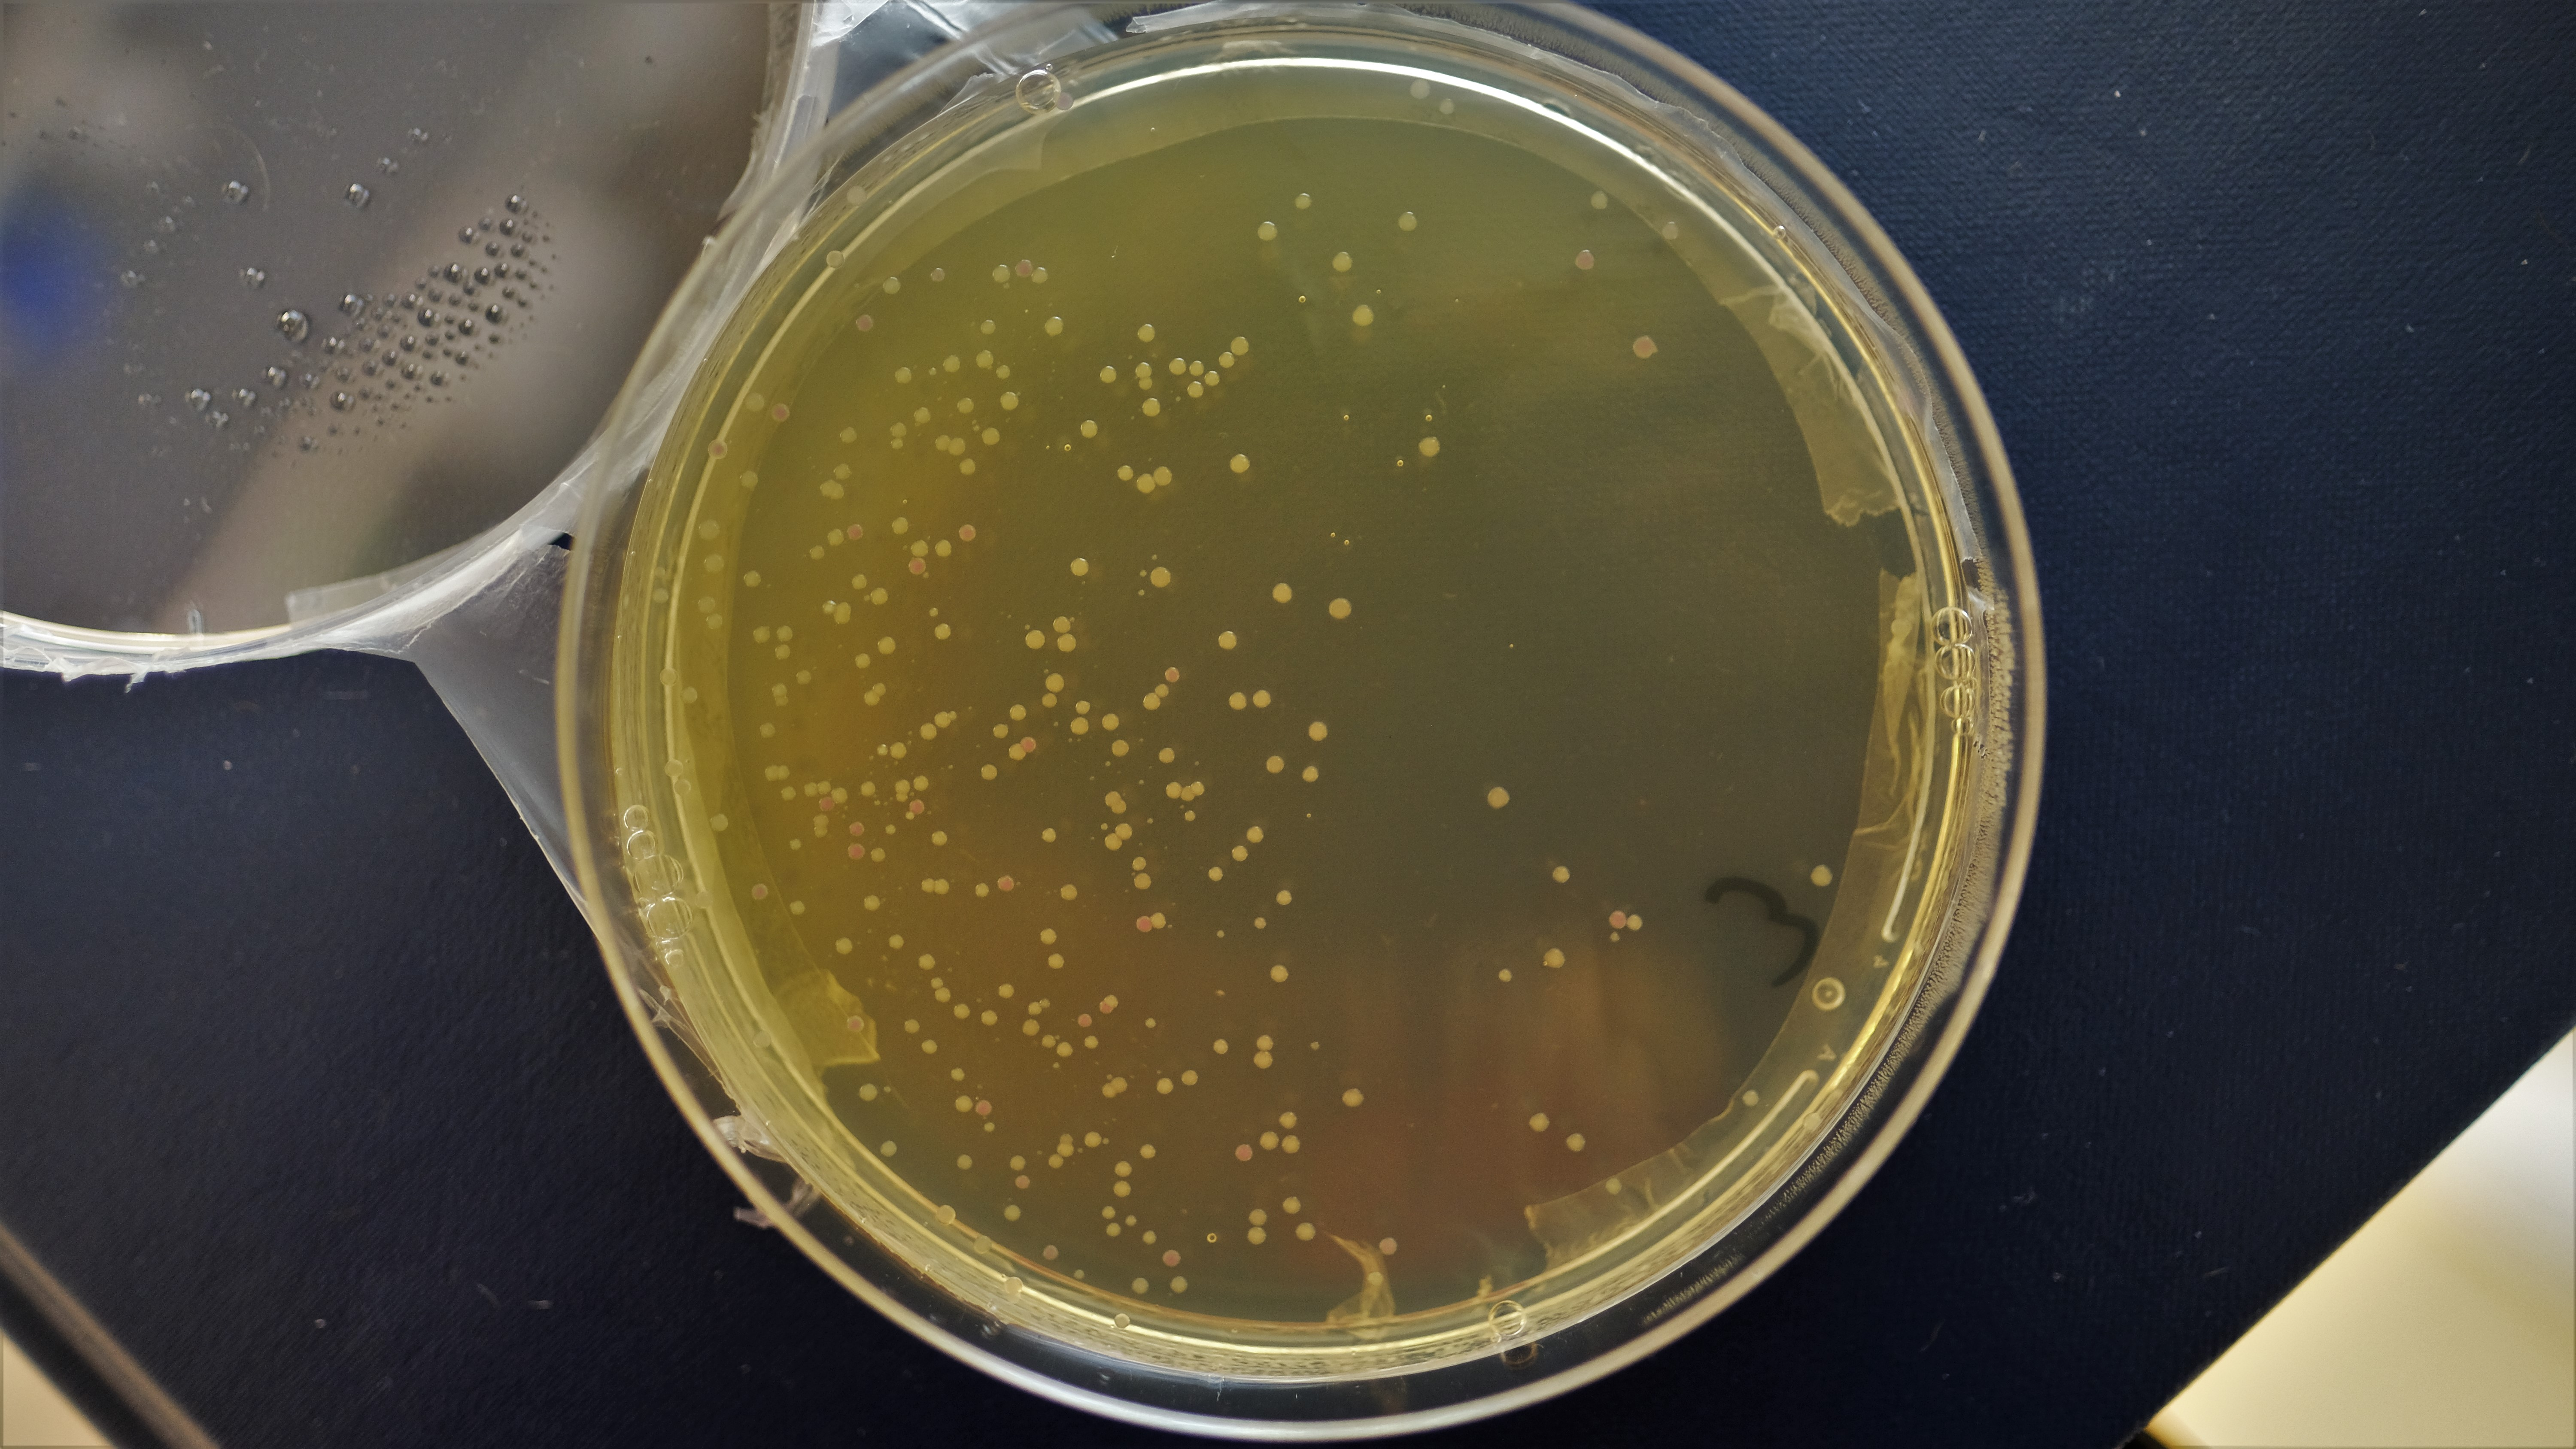
\includegraphics[scale=0.04]{Dellabb 4 kolonier redigerad.jpg}
    \caption{Result of incubation of transformed \textit{E. coli} cells}
    \label{fig:my_label}
\end{figure}

\subsection{PCR amplification}
The expected length of the amplicon was exactly 1232 bp based on the primers used in this lab. 1232 bp is located between the tenth (1500 bp) and eleventh (1200 bp) band on the DNA ladder (from top to bottom). This agrees with the height of the band of the right-most column. It is almost imperceptible, but the red colony shows a faint band at the same height. The mutation can be seen in Appendix D. 
\begin{figure}[H]
    \centering
    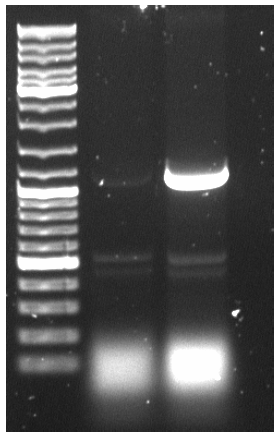
\includegraphics[scale=0.3]{Dellabb 6 DNA.png}
    \caption{Gel electrophoresis of whole colony under UV light. From left to right: DNA ladder, red colony, white colony}
    \label{colony pcr}
\end{figure}

\subsection{Sanger sequencing}
The sequencing showed that the stop codon TAA was successfully mutated to CAA in red colonies, see Appendix D. This was expected as primers used in the mutagenesis step had this mutation (mismatch). CAA codes for glutamine. 

The sequence from the white colony matches perfectly with that of the red colony which is natural as they should only differ in one basepair. They show increasingly inaccurate readings starting from the 700 region and are unrecognizable towards the end at 1000 bp with many unidentified nucleotides (N) and alignment errors compared to the reference strand. Sanger sequencing methods are accurate up to 750 bp for a single run (\cite{brown}), so this behaviour is expected. However, it is unclear as to why the sequencing data does not start at the sequencing primer end relative to the reference sequence.

\subsection{Protein production and analysis}
Lane 2 and 4 (from red colonies) both show intense bands at the size of 45 kDa (third band from the top on protein ladder), see Fig. 4. This was not expected as the size of the His$_6$-Z-mCherry protein is 36.8 kDa. 

All sample lanes show scattered and weak bands at similar regions, these are irrelevant proteins present in the cell lysate. It is interesting, however, to note how strongly the His$_6$-Z-mCherry fusion protein is expressed compared to the constitutional proteins. No IPTG nor lactose were present in the liquid medium to trigger the transcription, but the lac promoter is relatively leaky(\cite{labbkomp}).
\begin{figure}[H]
    \centering
    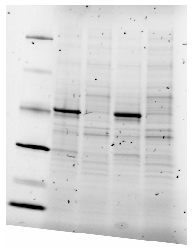
\includegraphics[scale=0.5]{Protein UV.png}
    \caption{SDS-PAGE analysis of protein. From the left: Protein ladder, red, white, red, white (colonies)}
    \label{sds}
\end{figure}
%------------------------------------------------------------------------------------

\section{Discussion}

In this lab, a mutation of the stop codon in the fusion protein His$_6$-Z-(stop)-mCherry was done through site-directed mutagenesis. To obtain a correct point mutation, an array of methods are used to both cause the mutation and to verify that the process is working accordingly. This lab gives insight to how well the different methods work in practice, their pros and cons, and also how to interpret the results.

Initially in the second part of the lab (electrophoresis analysis of plasmid extraction), the concentration of extracted expression-vector plasmids from the \textit{E. coli} is estimated through comparison to a "High DNA mass ladder" in electrophoresis. When merely observed, the bands from the plasmid can only be estimated to be less than 10 ng/$\mu$L in sample B, and around 100 ng/$\mu$L in sample A, which was incorrect when based on the results from the NanoDrop. This method is infeasible as exact measurements are desired (additionally, determining intensity by eye is not reliable). The bands of the ladders represent different concentrations and sizes of DNA, but a majority of the bands seem to be expressed in the same intensity when merely observed. The range of the concentrations represented by the DNA mass ladder bands is quite small. The only appropriate time to use the DNA ladder would be when very broad and non-exact bounds are needed. A NanoDrop spectrometer was used to calculate the concentration of the plasmid solution, and is a much preferred method. 

The amount of resulting colonies that expressed the desired His$_6$-Z-mCherry fusion protein, and as a result showed a red colour, was relatively low at a mutation frequency of 11 \% (Appendix B). This could be caused by a multiple of factors most likely introduced during the mutagenesis step of the pHis$_6$-Z-(stop)-mCherry plasmid (part 3 of the lab). Either too low concentrations of essential reactants like dNTP and forward-/reverse primers or too few cycles of PCR for mutagenesis could have resulted in less probability for the mutation to take place. Combining this with the low effectivity of the enzyme \textit{dpn}I, the factor of mutated plasmids amongst intact plasmids would be quite modest. 

In some settings, a low transformation frequency is not a problem as one can inoculate a colony with the desired transformation (in principle requiring only one successful transformation). However, in \textit{in vivo} medical applications, a high mutation frequency could be crucial for the efficiency of some gene editing based treatment. The frequency can be increased by developing the methods and correcting the few frequency decreasing factors mentioned earlier (e.g. higher concentration of primers and more PCR-cycles). The inefficiency of the enzyme \textit{dpn}I can be compensated by using a higher concentration and in the optimal working temperature of 37 $^\circ C$ (\cite{TF}). 

PCR was done on the resulting red and white colonies after transformation and inoculation to amplify a sequence around the mutation site. PCR is highly effective when it comes to amplifying a small sample of nucleotide sequences when needed in a larger quantity, but can introduce new mismatches which is a problem for the subsequent sequencing. There is also a risk of the primers binding to the incorrect site if they are too non-selective, but can be easily solved by using a longer oligonucleotide.

In part 6 of the lab, the PCR products were analysed through gel electrophoresis (Figure 3), this is redundant. The bands appear at the same height because the mutation is a point mutation, so there is no change in plasmid length. Even if the mutation would have been a deletion or insertion, a difference of one bp would not be visible nor give us the desired results since it would cause a frame shift on the downstream mCherry domain. The bands from the white colony was far weaker than the bands from the red colony. The reason for the very faint intensity of the bands from the white colony in Fig. \ref{colony pcr} is that it was done directly from a cell lysate solution whose concentration was not checked. To avoid this problem, one could run a NanoDrop test as in part 2 of the lab and adjust the concentration thereafter. Electrophoresis would be relevant to run if a sequence of detectable length was ligated into the plasmid.

In part 9 of the lab, the proteins produced by the mutated and non-mutated cells were analysed using SDS-PAGE. In the obtained electrophoresis results (Figure 3), the His$_6$-Z-mCherry fusion protein shows a relatively strong signal at 45 kDa when compared to the other bands in the lane. The cause for this strong band could be the leaky nature of the lac promoter regulating the transcription of the His$_6$-Z-mCherry gene (\cite{labbkomp}). The theoretical size of the fusion protein is slightly smaller (36.8 kDa) than the one shown on the SDS-PAGE (\cite{labbkomp}). A reason could be an inadequate amount of SDS used to even out the charges of all proteins, leading to bonding between some irrelevant proteins and the fusion protein. Even though the non-mutated protein His$_6$-Z is controlled by the same lac-promoter as the complete fusion protein, a band of similar intensity was not expected to be seen in lane 3 and 5 (ladders for the white inoculant) because His$_6$-Z has the size $36.8-26.7=10.1$ kDa which is less than the smallest band on the protein ladder (14 kDa). There is a possibility for the smaller protein to have migrated through the whole gel, and diffused into the conducting fluid and rendered undetectable under UV. 

When observing the large amount of expressed fusion protein even at complete absence of the inducer IPTG, one could deduce that it is inappropriate to use the lac promoter when trying to synthesize a toxin harmful to the cell, especially during growth. It would be preferable to use a promoter that is more strictly controlled.

Some of the methods used in this lab can be exchanged with more effective ones, and a higher mutation yield can always be achieved by adjusting some factors in each process, as has been discussed in this section. The resulting mutation frequency was at a mere 11 \%, but was obtained without any difficulty during practice. It is clear to see that every method introduced in this lab has its use for getting the correct point mutation desired, and to verify its occurrence.

\printbibliography[
heading=bibintoc,
title={References}
]

\pagebreak
\begin{center}

\section*{Appendix}\end{center}
\\
\appendix

 \section{Volume of DNA for mutagenesis}
$$V=\frac{m}{C_m}=\frac{700 \; ng}{170 \; ng/\mu L}=1.4 \; \mu L$$

 \section{Transformation frequency}
  \begin{table}[H]
\begin{center}
 \begin{tabular} {l|cc}
%\hline
 & Amount (\#) & Percentage (\%) \\
 \hline
 Transformed & 29 & $\frac{29}{262}=11$ \\ 
 Untransformed & 233 & $\frac{233}{262}=89$ \\  
 \hline
 $\sum$ & 262 & 100
\end{tabular}
\end{center}
\end{table}

 \section{Calculations for PCR reaction}
 We use $V_1=\frac{C_2}{C_1}V_2$ and $V_2=50 \; \mu L$:
  \begin{table}[H]
\begin{center}
 \begin{tabular} {c|c}
%\hline
Reagent & Volume ($\mu$L)\\
\hline
 dNTPs & $\frac{200 \; \mu M}{2\;mM}V_2=5 $ \\  
 Forward primer & \multirow{2}{*}{$\frac{5\;mol/\mu L}{0.5\; \mu M}V_2=5$} \\
 Reverse primer & \\
 10x PCR buffer & $\frac{1x}{10x}V_2=5$ \\
 Taq DNApol & $\frac{0.05\;U/\mu L}{5\;U/\mu L}V_2=0.5$ \\
 Cell lysate & 2 \\
 MilliQ & 50-17.5 = 32.5 \\
 \hline
 $\sum$ & 50
\end{tabular}
\end{center}
\end{table}

 \section{Sequencing results}
"X" was added in the start and end of white and red seqences due to issues with the \TeXshade $\:$ alignment shading tool. These should be ignored. The three sequences were aligned with EMBOSS Cons tool available \href{https://www.ebi.ac.uk/Tools/msa/emboss_cons/}{\textcolor{blue}{here}}. \\
\begin{texshade}{test2.fasta}
\shadingmode{similar}
\threshold[0]{100}
\setends{1}{00..2000}

\feature{bottom}{1}{414..414}{fill:$\uparrow$}{Mutation}
%\feature{top}{1}{220..230}{fill:$\downarrow$}{His$_6$ tag start}
\feature{top}{1}{216..233}{brace}{His$_6$ tag}
\feature{top}{1}{400..430}{<->[Black]}{Mutagenesis primers}
\feature{top}{1}{5..21}{l->[Black]}{PCR \& sequencing primer}
\feature{top}{1}{1198..1227}{<-l[Black]}{PCR primer, reverse}
%\feature{top}{1}{5..15}{fill:$\downarrow$}{His$_6$ tag end}
%\feature{top}{1}{302..304}{fill:$\downarrow$}{Mutation}
%\feature{top}{1}{302..304}{fill:$\downarrow$}{Mutagenesis primer backward}
%\feature{top}{1}{302..304}{fill:$\downarrow$}{Mutagenesis primer forward}

\hideconsensus
\end{texshade}

\section{Calculation of ampicillin needed for inoculation} 
$$
     C_1V_1=C_2(10 \;ml+V_1) \rightarrow V_1=0.1010\; \mu L 
     \label{ampicillin}
    $$
 
 \section{Peer review comments}
 All of Daniel Ullmans comments were relevant and well spotted and corrected, many thanks.
 
 Simona Pettersson is mistaken about report structure; the abstract is never given a number. It can be given a separate page before the TOC but we deem it unnecessary. Appendices can be lettered rather than numbered. Thanks for your kind comments.

\end{document}

 \begin{figure}[H]
     \centering
     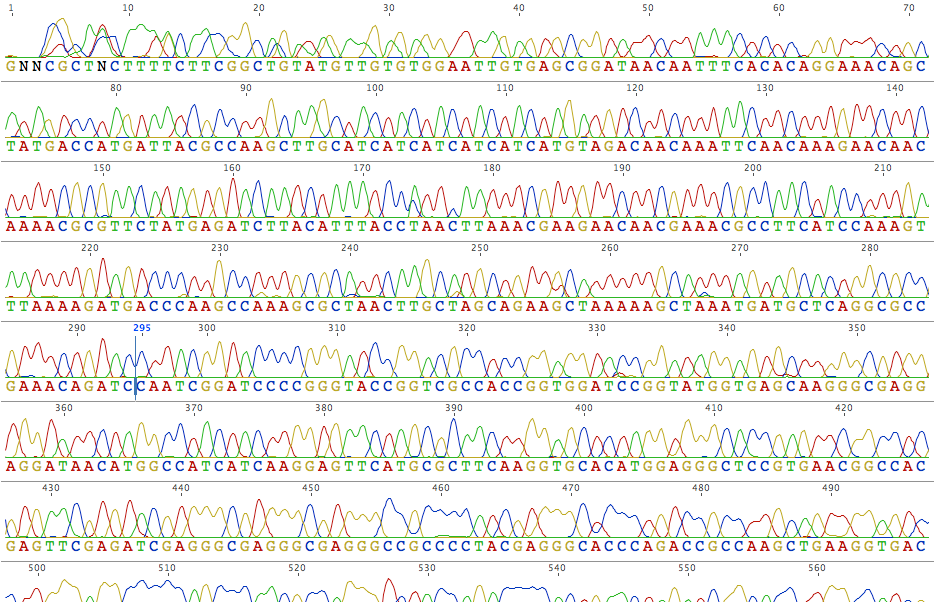
\includegraphics[scale=0.1]{Sangerseq.png}
     \caption{Sanger sequencing results}
     \label{fig:sanger}
 \end{figure}



\begin{table}[H]
\small
\begin{center}

\begin{tabular} { c c }
%\hline
Reagent & Volume ($\mu$L)\\
\hline
 Mutagenesis mixture & 40 \\ 
 10x CutSmart buffer & 5 \\  
 MilliQ & 4.5 \\
 \textit{Dpn}I enzyme (2U/$\mu$L) & 0.5 \\
 \hline
 $\sum$ & 50
\end{tabular}
\end{center}
\end{table}
